\chapter{Introducción}
\label{cap:capitulo1}
\setcounter{page}{1}

\begin{flushright}
\begin{minipage}[]{10cm}
\emph{La motivación nos impulsa a comenzar y el hábito nos permite continuar}\\
\end{minipage}\\

Jim Ryun\\
\end{flushright}

\vspace{1cm}

La robótica ha sufrido una transformación enorme a lo largo de su historia aunque siempre teniendo en mente el mismo objetivo: cumplir con el deseo humano. Debido a esa transformación y ese deseo, se ha podido consolidar este campo en la actualidad que abarca cada sector que se pueda imaginar. Otra vertiente que ha destacado en la robótica estos últimos años ha sido la creación de robots de bajo coste para que puedan llegar a un mayor número de personas y se puedan beneficiar de esta ciencia. 

En el presente capítulo se va a abordar el contexto de la robótica, explicando brevemente su historia para poder entender realmente qué es la robótica y lo que es un robot. También se van a encuadrar los tipos de robots que existen y sus múltiples aplicaciones. Todo esto nos ayudará a poder entender mejor dónde se encuadra el presente trabajo, proporcionando los conocimientos necesarios, tanto teóricos como prácticos, que se describirán a lo largo del documento.\\

\section{La robótica}
\label{sec:robotica} % etiqueta para luego referenciar esta sección

La robótica es el campo de la ingeniería que se enfoca en el diseño, la construcción y la programación de robots para tareas específicas. Por ende, un robot se podría definir como un sistema informático formado por sensores y actuadores imprecisos, ya que tienen ruido. Los robots realizan tareas sucias, aburridas y peligrosas y tienen que ser sensibles al entorno. Sin embargo, no existe una definición unívoca al respecto y depende del campo y de la época de la que queramos hablar. Para poder entenderlo, se va a hacer un breve resumen sobre la historia de la robótica.\\

Desde la antigüedad se han desarrollado ingenios o autómatas de los cuáles muchos de ellos tenían fines religiosos  muestra la Figura \ref{fig:ancientrel}.   \\


\begin{figure}[ht!]
	\centering
	\begin{minipage}{0.4\linewidth}
		\centering
		\includegraphics[width=\linewidth]{figs/memnon.jpeg}
		\caption*{\centering Estatuas de Memnon} %\cite{memnon_image}
	\end{minipage}
	\hspace{2cm}
	% aquí incluir iamgen de Guerrero de terracota
	\begin{minipage}{0.35\linewidth}
		\centering
		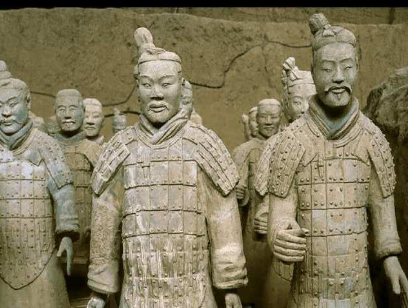
\includegraphics[width=\linewidth]{figs/terracota.png}
		\caption*{\centering Guerreros de Terracota} %\cite{gomezguerreros}
	\end{minipage}
	\caption{Ingenios de la antigüedad con fines religiosos}
	\label{fig:ancientrel}
\end{figure}

 
Otras invenciones que destacaban por otras aplicaciones fueron el tornillo de Arquímedes de Siracusa, la eolípila de Herón de Alejandría, el ornitóptero de Leonardo Da Vinci y el hombre de palo de Juanelo Turriano, entre otras. Se pueden apreciar algunas de dichas invenciones en la Figura \ref{fig:ancient}.\\

En \cite{cuenca2023diseno} se trata el principio de generación hidroeléctrica, tomando en cuenta el modelo tornillo de Arquímedes. También en el artículo \cite{giri2020maquinas} se traza una línea histórica de las máquinas térmicas, teniendo en cuenta a la eolípila. 

\begin{figure}[ht!]
	\centering
	% Imagen del tornillo de Arquímedes de Siracusa
	\begin{minipage}{0.3\linewidth}
		\centering
		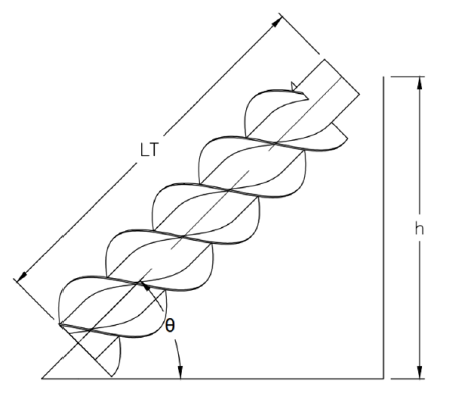
\includegraphics[width=\linewidth]{figs/arquimedes.png}
		\caption*{\centering Tornillo de Arquímedes}  %\cite{cuenca2023diseno}
	\end{minipage}
	\hspace{3cm}
	% Imagen de la eolípila
	\begin{minipage}{0.3\linewidth}
		\centering
		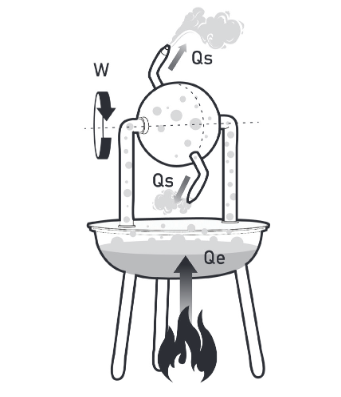
\includegraphics[width=\linewidth]{figs/eolipila.png}
		\caption*{\centering Eolípila} %\cite{giri2020maquinas}
	\end{minipage}
	%\hspace{3cm}
	% Imgen del ornitóptero
	%\begin{minipage}{0.3\linewidth}
	%	\centering
	%	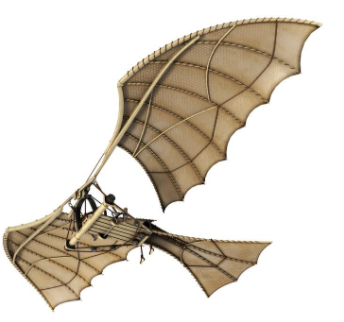
\includegraphics[width=\linewidth]{figs/davinci.png}
	%	\caption*{\centering Ornitóptero \cite{velazquezcual}}
	%\end{minipage}
	%\hspace{3cm}
	% Imagen del hombre de palo 
	%\begin{minipage}{0.3\linewidth}
	%	\centering
	%	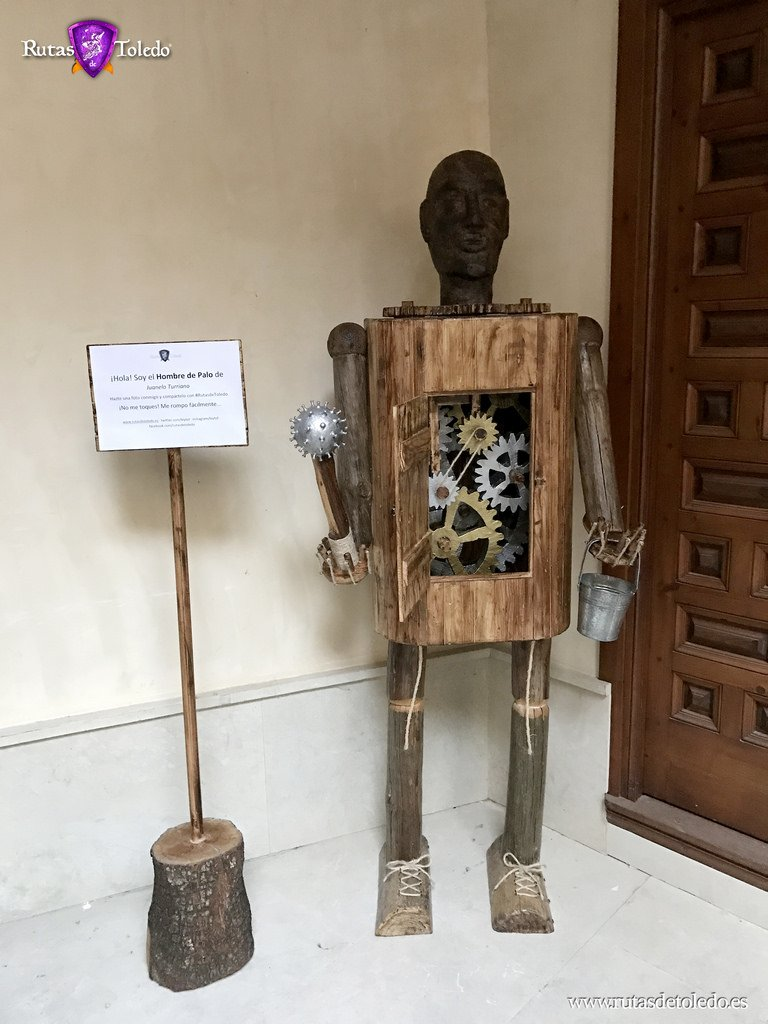
\includegraphics[width=\linewidth]{figs/hombre-palo.jpg}
	%	\caption*{\centering Hombre de palo \cite{hombredepalo_leyendasdetoledo}}
	%\end{minipage}
	\caption{Ingenios de la antigüedad con fines no religiosos}
    \label{fig:ancient}
    \end{figure}

Durante el siglo XX la ciencia dejó de ser una actividad desarrollada en aislamiento y se desarrolló en laboratorios con más gente. El movimiento del positivismo lógico fomentó las investigaciones ya que este movimiento trataba de dar importancia a la ciencia y dejar de lado la filosofía; también, el contexto de las guerras mundiales y de las bombas nucleares influyeron significativamente en este aspecto. Ya se empieza a acuñar la palabra robot y surge Electro y Sparko de Westinghouse Electric Corporation (Figura \ref{fig:EyS}), tratado en muchas ocasiones como uno de los primeros robots, como se describe en \cite{bidaudrobots}. Un descubrimiento muy destacado fue y sigue siendo hoy en día son Las Leyes de la Robótica de Isaac Asimov (Figura \ref{fig:Asimov}), así lo transmite \cite{barcelo2004nuevo}.\\


\begin{figure} [h!]
	\begin{center}
		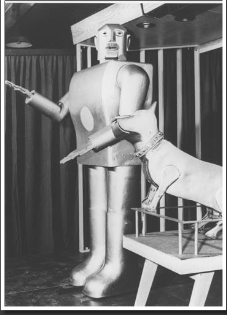
\includegraphics[width=8cm]{figs/electro-sparko.png}
	\end{center}
	\caption{Electro y Sparko} %\cite{bidaudrobots}}
	\label{fig:EyS}
\end{figure}

\begin{figure} [h!]
	\begin{center}
		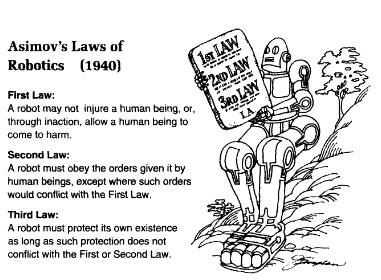
\includegraphics[width=12cm]{figs/issac-law.png}
	\end{center}
	\caption{ Leyes de la robótica} %\cite{barcelo2004nuevo}
\label{fig:Asimov}
\end{figure}


%\ac{} expande las siglas
%\acs{} no expande las siglas
\cite{nilsson1984shakey} nos cuenta que en 1969 se construye por el \ac{SRI} Internacional un prototipo experimental llamado Shakey que era una unidad independiente de 1.5 metros, equipado con 2 motores, cámara de televisión y una radio conectada a un ordenador, capaz de navegar en entornos cerrados y estructurados de una forma autónoma. Sus objetivos eran aprender del medio y ser capaz de planificar trayectorias de movimiento y las tareas que le asignaron fueron mover y detectar bloques. Sin embargo, cada movimiento podría tardar más de una hora en computarse y aún así, podrían producirse fallos. A Shakey se le conoce como el primer robot móvil (Figura \ref{fig:shakey}). \\

\begin{figure} [h!]
	\begin{center}
		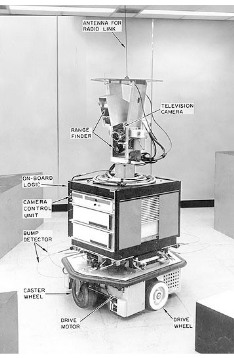
\includegraphics[width=8cm]{figs/shakey.png}
	\end{center}
	\caption{Robot Shakey} %\cite{nilsson1984shakey}}
	\label{fig:shakey}
\end{figure}\


Otro robot muy conocido  y descrito en \cite{earnest2012stanfordcart} es la carreta de Stanford que era capaz de ver y moverse en cualquier ambiente. Con la cámara que disponía, era capaz de calcular y trazar distancias. Sin embargo, tardaba 5 horas en recorrer 30 metros (Figura \ref{fig:stanford}). 

\begin{figure} [h!]
	\begin{center}
		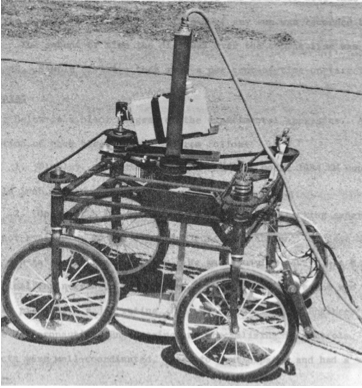
\includegraphics[width=8cm]{figs/stanford.png}
	\end{center}
	\caption{Carreta de Stanford}
	\label{fig:stanford}
\end{figure}\


Ya a partir de la década de los 80, se decidió que el acceso a los robots fuese para todo el mundo. Lo que provocó asombro, inquietud y miedo ya que el desconocimiento de aquella situación generó rechazo; cosa que ocurre hoy en día. El mundo de la literatura y cine tampoco ayudaba en ese aspecto ya que se presentaba al robot como algo perjudicial para la humanidad. Afortunadamente, esta situación va menguando con el tiempo y se está consiguiendo ver a los robots como un asistente del ser humano que lo que quiere es mejorar su calidad de vida. Para conocer en qué ámbitos un robot puede ayudar al ser humano, es necesario conocer que se clasifican en robots industriales y de servicio. \\


\subsection{Robots industriales}

Los robots industriales son brazos robotizados y manipuladores que tienen más de tres grados de libertad, trabajan en entornos controlados y usan efectores como: pinzas, ventosas. etc. Usan control por posición y planificación de trayectorias para poder controlar dichos brazos y poder realizar operaciones como \textit{pick and place}, ensamble de piezas, entre otros. Una variante de los robots industriales son los cobots: capaces de interactuar y colaborar con humanos. Dentro del mercado de los robots industriales se puede ver que tiene proveedores asentados como \acs{KUKA} o \acs{ABB} (Figura \ref{fig:robindustriales}).


%\begin{figure}[ht!]
%	\centering
%	\begin{minipage}{0.3\linewidth}
%		\centering´
%		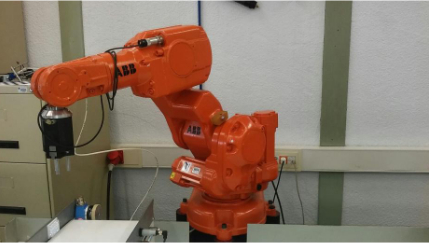
\includegraphics[width=\linewidth]{figs/brazoIRB140.png}
%		\caption*{\centering Brazo robot IRB 140 } % \cite{villalba2017ensamblaje}}
%	\end{minipage}
%	\hspace{3cm}
	% aquí incluir iamgen de Guerrero de terracota
%	\begin{minipage}{0.3\linewidth}
%		\centering
%		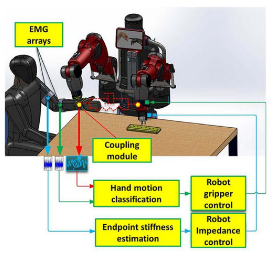
\includegraphics[width=\linewidth]{figs/cobot.png}
%		\caption*{\centering Cobot \cite{ELZAATARI2019162}}
%	\end{minipage}
%	\caption{Robots industriales}
%\end{figure}



\begin{figure}[ht!]
	\centering
	\begin{minipage}{0.3\linewidth}
		\centering
		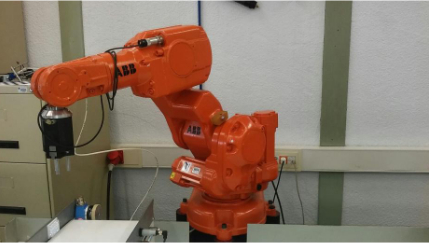
\includegraphics[width=\linewidth]{figs/brazoIRB140.png}
		%\caption*{\centering Brazo robot IRB 140 \footnote{{\url{https://www.youtube.com/watch?v=BBrLAOr89KY}}}}
		%\caption*{Brazo robot IRB 140~\ref{note:enlace1}.}
		\caption*{Brazo robot IRB 140~\footnotemark[1]}

	\end{minipage}
	\hspace{3cm}
	\begin{minipage}{0.3\linewidth}
		\centering
		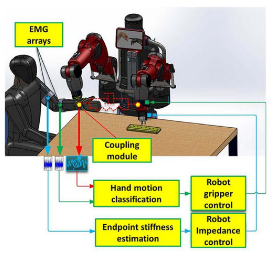
\includegraphics[width=\linewidth]{figs/cobot.png}
		%\caption*{\centering Cobot \cite{ELZAATARI2019162}}
		%\caption*{Cobot $^{\footnotesize{\ref{note:enlace2}}}$.}
		\caption*{Cobot $^{\ref{note:enlace2}}$.}
		
	\end{minipage}
	\caption{Robots industriales}
	\label{fig:robindustriales}
\end{figure}


\footnotetext[1]{\url{https://www.youtube.com/watch?v=BBrLAOr89KY}}
%\footnotetext[1]{\url{https://www.youtube.com/watch?v=BBrLAOr89KY}}


%\renewcommand{\thefootnote}{\textsuperscript{\smaller\arabic{footnote}}} % Cambiar el tamaño del número de la nota al pie
% Definir la primera nota al pie con el número 1
%\setcounter{footnote}{1} % Reiniciar la numeración de notas al pie
%\renewcommand{\thefootnote}{\textsuperscript{\smaller\arabic{footnote}}} % Cambiar el tamaño del número de la nota al pie
%\footnotetext[\value{footnote}]{\url{https://www.youtube.com/watch?v=BBrLAOr89KY}\label{note:enlace1}}

% Definir la segunda nota al pie con el número 2
\setcounter{footnote}{2} % Establecer la numeración de la siguiente nota al pie
\footnotetext[\value{footnote}]{\href{http://www.ejemplo2.com}{http://www.ejemplo2.com}\label{note:enlace2}}


\subsection{Robots de servicio}

Los robots de servicios son todos aquellos que no son industriales; por lo tanto, tienen menos de 3 grados de libertad, no trabajan en un entorno controlado, son más difíciles de programar, toman aplicaciones heterogéneas y todavía se encuentran en un mercado inmaduro. Existen muchos tipos de robots de servicio, de los cuáles a continuación se podrán enumerar algunos campos con algunos de sus respectivos ejemplos. \\ 


\subsubsection{Robots de limpieza}

En \cite{plaza_robotica_servicio} se define a los robots de limpieza como aquellos robots que se encargan de eliminar la suciedad. Dependiendo de sus características, pueden ser capaces de aspirar y fregar el suelo, o de limpiar los cristales de las ventanas. Estos últimos, son comunes en edificios que tienen grandes ventanales y un difícil acceso a ellos. Las aspiradoras se encuentran en un mercado mundial asentado cuyos inicios eran aspiradoras que usaban sensores de contacto, encoders y una navegación pseudoaleatoria (Figura \ref{fig:roblimpieza} izquierda); y han evolucionado hasta el punto de usar mapas para poder navegar y poder localizarse. También, usan algoritmos sofisticados como navegación de cobertura por barridos sistemáticos \acs{BSA} y se componen de sensores más sofisticados como láseres y cámaras que son capaces de detectar obstáculos como calcetines y ser capaz de esquivarlos (Figura \ref{fig:roblimpieza} derecha).\\


\begin{figure}[ht!]
	\centering
	\begin{minipage}{0.3\linewidth}
		\centering
		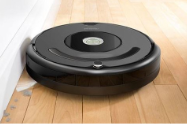
\includegraphics[width=\linewidth]{figs/gama-baja.png}
		\caption*{\centering Modelo económico }% \cite{plaza_robotica_servicio}}
	\end{minipage}
	\hspace{3cm}
	% aquí incluir iamgen de Guerrero de terracota
	\begin{minipage}{0.3\linewidth}
		\centering
		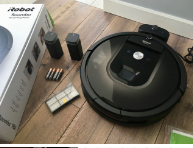
\includegraphics[width=\linewidth]{figs/gama-alta.png}
		\caption*{\centering Gama alta} % \cite{plaza_robotica_servicio}}
	\end{minipage}
	\caption{Robots de limpieza}
	\label{fig:roblimpieza}
\end{figure}


\subsubsection{Robots de entretenimiento}

Son aquellos robots que tienen aplicaciones heterogéneas en un mercado educativo asentado pero también existen muchos prototipos sin un uso comercial claro. En la educación, se ha ido introduciendo la robótica de manera muy atractiva y didáctica a los estudiantes hasta el punto de conseguir tener una asignatura destinada a la robótica y poder participar en competiciones como: \ac{FLL}, Robocup Junior y Robocampeones, entre otros (Figura \ref{fig:robed} izquierda).  En dicha asignatura se adquieren conocimientos generales de programación, impresión 3D, lógica, introducción a la electrónica y los microcontroladores.

Los prototipos nombrados anteriormente suelen ser demostradores tecnológicos que se crean para exhibiciones, se encuentran a la vanguardia de la tecnología y sirven para atraer un mayor número de clientes como puede ser: Spot de Boston Dynamics, Pepper de Softbank o Sophia de Hanson Robotics. En la Figura \ref{fig:robed} (derecha) se pueden ver un ejemplo de estos demostradores.\\


\begin{figure}[ht!]
	\centering
	\begin{minipage}{0.3\linewidth}
		\centering
		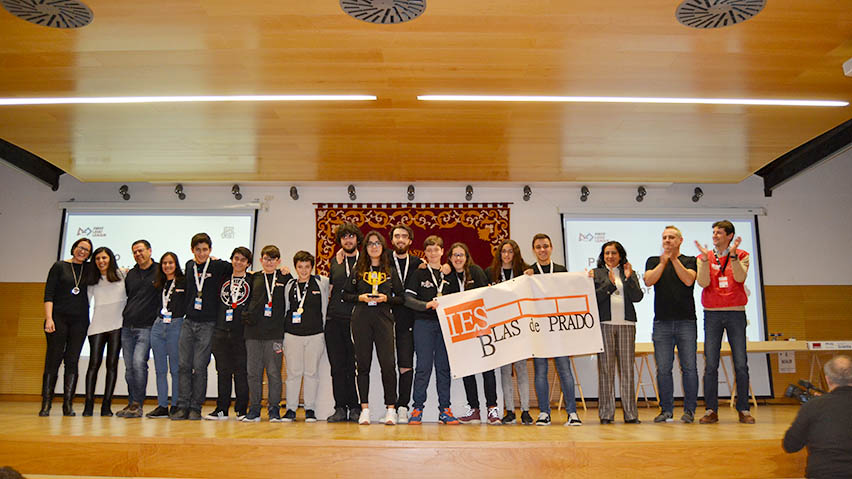
\includegraphics[width=\linewidth]{figs/FLL_TO19.jpg}
		\caption*{\centering\href{https://www.uclm.es/noticias/febrero2019/toledo/finalfirstlegoleague}{Competición \ac{FLL} Toledo} }
	\end{minipage}
	\hspace{3cm}
	% aquí incluir imagen de Spot
	\begin{minipage}{0.3\linewidth}
		\centering
		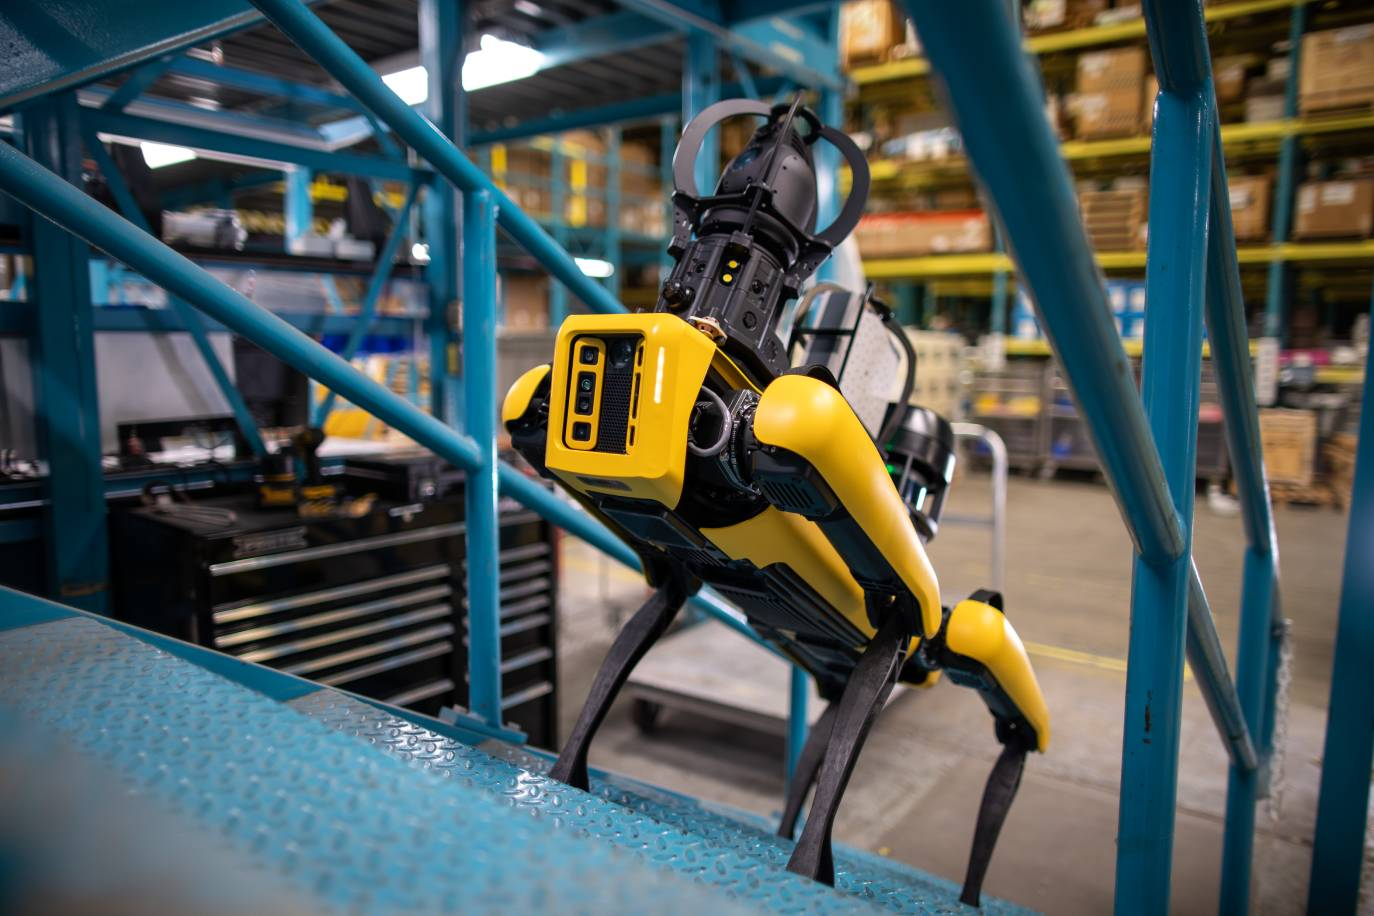
\includegraphics[width=\linewidth]{figs/spot.jpg}
		\caption*{\centering\href{https://bostondynamics.com/products/spot/}{Spot de Boston Dynamics}}
	\end{minipage}
	\caption{Robótica enfocada al entretenimiento}
	\label{fig:robed}
\end{figure}


\subsubsection{Robots de salud}

Los robots de salud sirven para mejorar la calidad de la atención médica y apoyar a los profesionales de la salud en diversas tareas. De esas tareas se pueden enumerar las siguientes: telepresencia, asistentes personales, cirugía, desinfección, esterilización, transporte interno y rehabilitación. De este gran abanico de tareas se puede destacar algunas aplicaciones que se puede ver en la Figura \ref{fig:robsalud}.\\

\begin{figure}[ht!]
	\centering
	\begin{minipage}{0.5\linewidth}
		\centering
		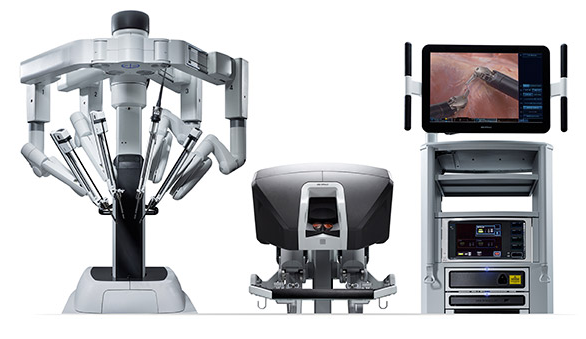
\includegraphics[width=\linewidth]{figs/davincimed.png}
		\caption*{\centering\href{https://www.abexsl.es/es/sistema-robotico-da-vinci/que-es}{Robot Da Vinci}}
	\end{minipage}
    \hspace{1 cm}
	% aquí incluir imagen de  mako
	\begin{minipage}{0.15\linewidth}
		\centering
		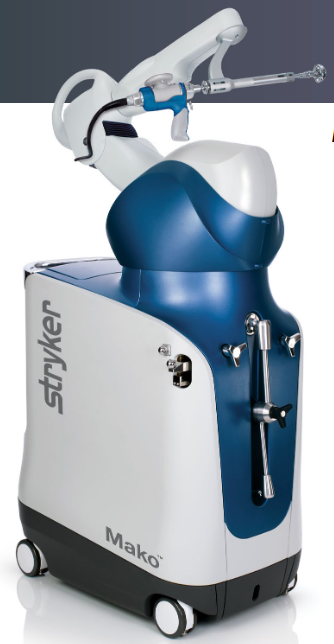
\includegraphics[width=\linewidth]{figs/mako.png}
		\caption*{\centering\href{https://www.stryker.com/content/dam/stryker/joint-replacement/systems/mako-system-overview/resources}{Robot Mako}}
	\end{minipage}
    \hspace{3cm}
    \begin{minipage}{0.2\linewidth}
    	\centering
    	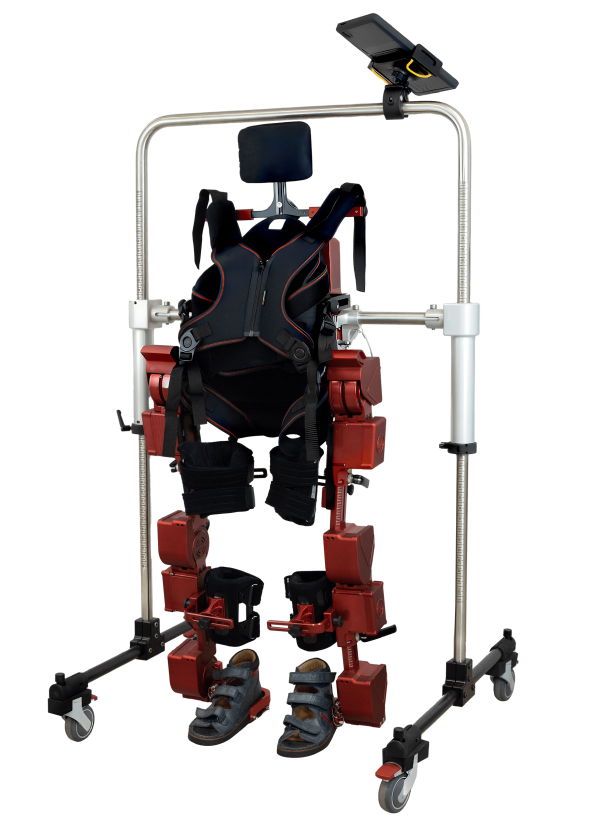
\includegraphics[width=\linewidth]{figs/marsi.png}
    	\caption*{\centering\href{https://www.marsibionics.com/}{Marsi Bionics} }
    \end{minipage}
    \hspace{3cm}
    \begin{minipage}{0.25\linewidth}
    	\centering
    	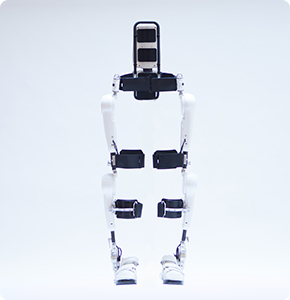
\includegraphics[width=\linewidth]{figs/cyberdyne.jpg}
    	\caption*{\centering\href{https://www.cyberdyne.com/}{CyberDyne}}
    \end{minipage}
	\caption{Robots de salud}
	\label{fig:robsalud}
\end{figure}

\subsubsection{Robots de logística}

Los robots de logística son sistemas automatizados diseñados para mejorar la eficiencia, precisión y velocidad en la gestión de la cadena de suministro y operaciones logísticas en cadenas de montaje y almacenes. Generalmente los sistemas automatizados son flotas de robots a las que se les aplica distintas arquitecturas software como puede ser \acs{AGV} o \acs{AMR} para poder realizar la tarea asignada. También existen prototipos de robots de reparto que son capaces de hacer entrega de última milla. La Figura \ref{fig:robreparto}  muestra ejemplos de robots de reparto. \\ 

\begin{figure}[ht!]
	\centering
	\begin{minipage}{0.3\linewidth}
		\centering
		\includegraphics[width=\linewidth]{figs/skypod.png}
		\caption*{\centering\href{https://exotecbydexter.com/skypod/}{Skypod de Exotec} }
	\end{minipage}
	\hspace{3cm}
	% aquí incluir imagen de Amazon prime air
	\begin{minipage}{0.3\linewidth}
		\centering
		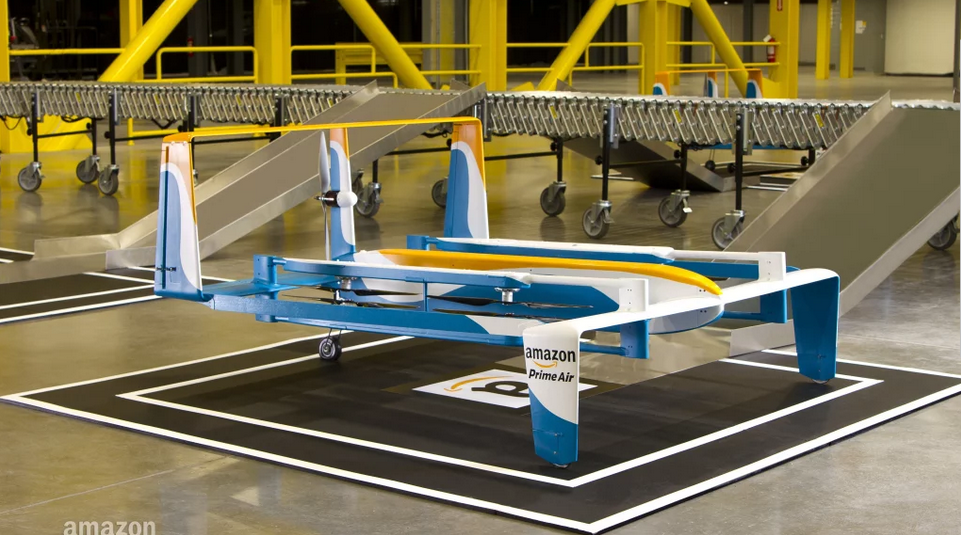
\includegraphics[width=\linewidth]{figs/amazon.png}
		\caption*{\centering\href{https://www.aboutamazon.es/noticias/innovacion/prime-air}{Amazon Prime Air}}
	\end{minipage}
	\caption{Robots de logística}
	\label{fig:robreparto}
\end{figure}

\section{Robots de campo}

En \cite{thorpe2003field} se define a los robots de campo como la automatización de muchas plataformas terrestres, marítimas y aéreas en aplicaciones como la minería, la manipulación de carga, la agricultura, la exploración y explotación submarina, las carreteras, la exploración planetaria, la vigilancia costera y el rescate, entre otros. La robótica de campo se caracteriza por la aplicación de los principios robóticos más avanzados en cuanto a sensado, control y razonamiento en entornos no estructurados y difíciles. El atractivo de la robótica de campo es que es una ciencia desafiante, involucra los últimos principios de ingeniería y diseño de sistemas, y ofrece la verdadera posibilidad de que los principios robóticos hagan una contribución económica y social sustancial en muchas áreas de aplicación diferentes. En general, los robots de campo son plataformas móviles que trabajan al aire libre, a menudo produciendo interacciones fuertes con sus entornos, sin supervisión humana.

En los últimos años se ha podido notar un gran progreso en el desarrollo y la implementación de sistemas robóticos de campo. En la Figura \ref{fig:robcampo} se pueden ver ejemplos al respecto. \\


\begin{figure}[ht!]
	\centering
	\begin{minipage}{0.3\linewidth}
		\centering
		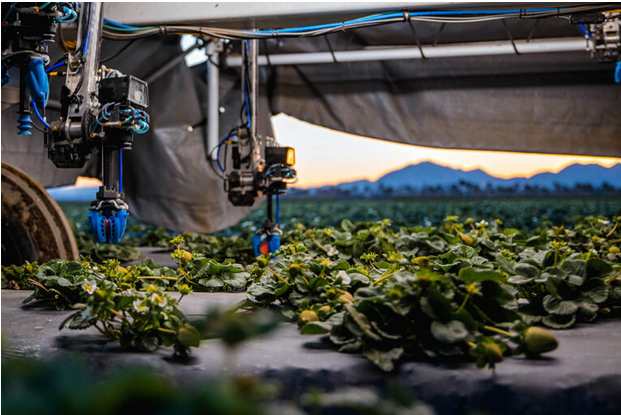
\includegraphics[width=\linewidth]{figs/strawberry.png}
		\caption*{\centering\href{https://advanced.farm/technology/strawberry-harvester/}{TX Robotic Strawberry Harvester}}
	\end{minipage}
	\hspace{3 cm}
	% aquí incluir imagen de  mako
	\begin{minipage}{0.3\linewidth}
		\centering
		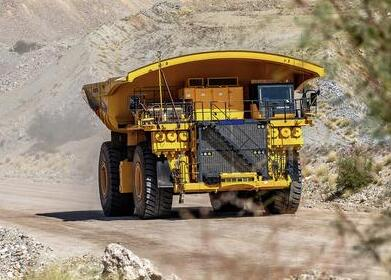
\includegraphics[width=\linewidth]{figs/komatsu.jpeg}
		\caption*{\centering\href{https://www.komatsu.com/en/technology/smart-mining/loading-and-haulage/autonomous-haulage-system/}{FrontRunner Autonomous Haulage System (AHS)}}
	\end{minipage}
	\hspace{3cm}
	\begin{minipage}{0.3\linewidth}
		\centering
		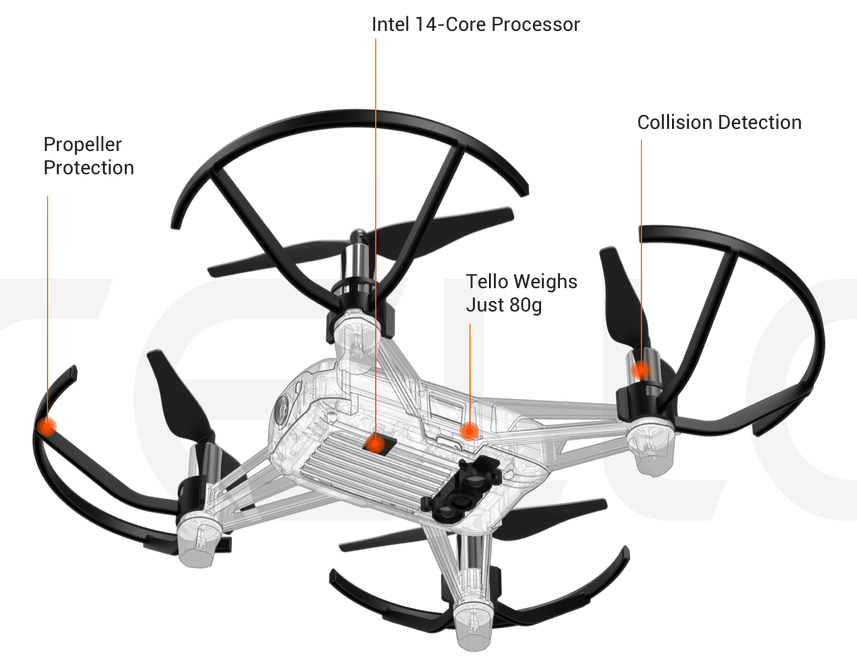
\includegraphics[width=\linewidth]{figs/tello.png}
		\caption*{\centering\href{https://www.ryzerobotics.com/es/tello}{Drone Tello}}
	\end{minipage}
	\hspace{3cm}
	\begin{minipage}{0.3\linewidth}
		\centering
		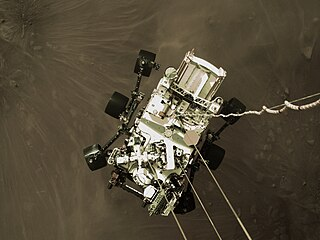
\includegraphics[width=\linewidth]{figs/perseverance.jpg}
		\caption*{\centering\href{https://es.wikipedia.org/wiki/Perseverance}{Perseverance}}
	\end{minipage}
	\caption{Robots de campo}
	\label{fig:robcampo}
\end{figure}

Por contra, debido a las condiciones que se tienen que someter estos robots, su coste es elevado e imposibilita que su uso se pueda extender a aquellos lugares que necesiten de su servicio y que tienen bajos recursos. Es por esto que existe una necesidad que para ciertas aplicaciones, que no tienen condiciones tan extremas, se creen robots asequibles que puedan lidiar con ciertas tareas. \\

\section{Robots de bajo coste}

Los robots de bajo coste son aquellos robots diseñados y fabricados con el objetivo de ser económicos, accesibles y fáciles de producir. Estos robots suelen emplear componentes menos costosos y métodos de fabricación simplificados para reducir el precio final. Algunas características clave de los robots de bajo coste incluyen:

\begin{itemize}
	\item \textit{Componentes asequibles}. Utilizan materiales y componentes electrónicos más baratos, como puden ser: motores de bajo coste como Parallax, microcontroladores como Arduino y ordenadores monoplaca como Raspberry pi.
	\item \textit{Simplicidad en el diseño}. Tienen diseños más sencillos que han sido creados usando técnicas de diseño e impresión 3D, facilitando su actualización y mantenimiento.
	\item \textit{Accesibilidad}. Están diseñados para ser utilizados por cualquier tipo de persona, sin tener una formación avanzada de la materia.
	\item \textit{Educación y prototipos}. Ampliamente usados en educación para facilitar el aprendizaje y también en la creación de prototipos rápidos y asequibles.
	\item \textit{Versatilidad}. Se adaptan a numerosas aplicaciones, desde las más sencillas hasta a proyectos más complejos.
	
\end{itemize}\

En resumen, los robots de bajo coste permiten la democratización de la tecnología robótica, facilitando su acceso a un público más amplio y fomentando la innovación y el aprendizaje en diferentes campos. En la Figura \ref{fig:roblowcost} se puede apreciar una aplicación real reciente de la robótica de bajo coste de la universidad \textit{Carnegie Mellon} descrita en el artículo \cite{shaw2024leap}.\\ 

\begin{figure} [h!]
	\begin{center}
		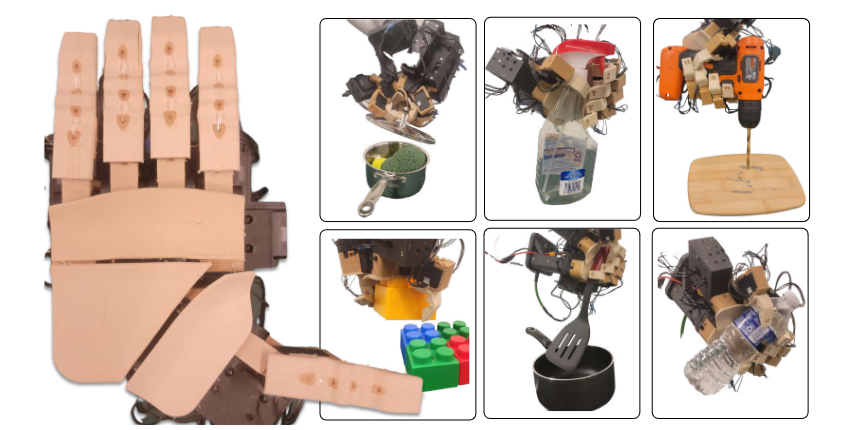
\includegraphics[width=16cm]{figs/handlowcost.png}
	\end{center}
	\caption{Mano Antropomórfica Híbrida Rígida y Suave} %\cite{shaw2024leap}}
	\label{fig:roblowcost}
\end{figure}\

El presente proyecto trata ....\\


Después de aquí pasar al aparatado del estado del arte \\\\

En los textos puedes poner palabras en \textit{cursiva}, para aquellas expresiones en sentido \textit{figurado}, palabras como \textit{robota}, que está fuera del diccionario castellano, o bien para resaltar palabras de una colección: \textit{(a)} es la primera letra del abecedario, \textit{(b)} es la segunda, etc.\\

Al poner las dos líneas del anterior párrafo, este aparecerá separado del anterior. Si no las pongo, los párrafos aparecerán pegados. Sigue el criterio que consideres más oportuno.

\section{Segunda sección}
\label{sec:segundaseccion}

No olvides incluir imágenes y referenciarlas, como la Figura \ref{fig:roomba}.

\begin{figure} [h!]
  \begin{center}
    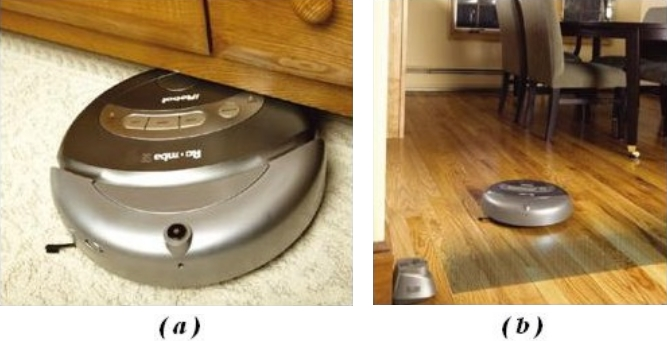
\includegraphics[width=8cm]{figs/roomba}
  \end{center}
  \caption{Robot aspirador Roomba de iRobot.}
  \label{fig:roomba}
\end{figure}\

Ni tampoco olvides de poner las URLs como notas al pie. Por ejemplo, si hablo de la Robocup\footnote{\url{http://www.robocup.org}}.

\subsection{Números}
\label{sec:subseccion}

En lugar de tener secciones interminables, como la Sección \ref{sec:robotica}, divídelas en subsecciones.

Para hablar de números, mételos en el entorno \textit{math} de \LaTeX, por ejemplo, $1.5Kg$. También puedes usar el símbolo del Euro como aquí: 1.500\euro.

\subsection{Listas}

Cuando describas una colección, usa \texttt{itemize} para ítems o \texttt{enumerate} para enumerados. Por ejemplo:

\begin{itemize}
 \item \textit{Entorno de simulación.} Hemos usado dos entornos de simulación: uno en 3D y otro en 2D.
 \item \textit{Entornos reales.} Dentro del campus, hemos realizado experimentos en Biblioteca y en el edificio de Gestión.
\end{itemize}\

\begin{enumerate}
 \item Primer elemento de la colección.
 \item Segundo elemento de la colección.
\end{enumerate}\

\paragraph{Referencias bibliográficas}
\label{sec:referencias}

Cita, sobre todo en este capítulo, referencias bibliográficas que respalden tu argumento. Para citarlas basta con poner la instrucción \verb|\cite| con el identificador de la cita. Por ejemplo: libros como \cite{vega12e}, artículos como \cite{vega19b}, URLs como \cite{vega19a}, tesis como \cite{vega18b}, congresos como \cite{vega18a}, u otros trabajos fin de grado como \cite{vega08b}.

Las referencias, con todo su contenido, están recogidas en el fichero \texttt{bibliografia.bib}. El contenido de estas referencias está en formato \texttt{BibTex}. Este formato se puede obtener en muchas ocasiones directamente, desde plataformas como \texttt{Google Scholar} u otros repositorios de recursos científicos.

Existen numerosos estilos para reflejar una referencia bibliográfica. El estilo establecido por defecto en este documento es APA, que es uno de los estilos más comunes, pero lo puedes modificar en el archivo \texttt{memoria.tex}; concretamente, cambiando el campo \verb|apalike| a otro en la instrucción \verb|\bibliographystyle{apalike}|. 

\

\

\

Y, para terminar este capítulo, resume brevemente qué vas a contar en los siguientes.
